\PassOptionsToPackage{svgnames}{xcolor}
\documentclass[11pt]{article}



\usepackage[margin=0in]{geometry}  
\usepackage{graphicx}             
\usepackage{amsmath}              
\usepackage{amsfonts}              
\usepackage{framed}               
\usepackage{amssymb}
\usepackage{array}
\usepackage{amsthm}
\usepackage{multirow}
\usepackage[nottoc]{tocbibind}
\usepackage{bm}
\usepackage[object=vectorian]{pgfornament} 
\usepackage{enumitem}
\usepackage{tikz}
\usepackage{minted}

\usetikzlibrary{shapes,arrows,positioning}
\colorlet{shadecolor}{lightgray!25}
\newcommand{\sectionline}{%
  \noindent
  \begin{center}
  {\color{DarkViolet}
    \resizebox{0.5\linewidth}{1ex}
    {{%
    {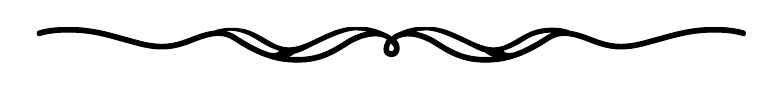
\begin{tikzpicture}
    \node  (C) at (0,0) {};
    \node (D) at (9,0) {};
    \path (C) to [ornament=85] (D);
    \end{tikzpicture}}}}}%
    \end{center}
  }

  \newcommand\norm[1]{\left\lVert#1\right\rVert}
\setlength{\parindent}{0cm}
\setlength{\parskip}{0em}
\newcommand{\Lim}[1]{\raisebox{0.5ex}{\scalebox{0.8}{$\displaystyle \lim_{#1}\;$}}}
\newtheorem{definition}{Definition}[section]
\newtheorem{theorem}{Theorem}[section]
\newtheorem{notation}{Notation}[section]
\theoremstyle{definition}
\DeclareMathOperator{\arcsec}{arcsec}
\DeclareMathOperator{\arccot}{arccot}
\DeclareMathOperator{\arccsc}{arccsc}
\DeclareMathOperator{\spn}{Span}
\setcounter{tocdepth}{1}
\begin{document}

%\twocolumn
\begin{minted}{java}
//BST.java
import java.util.NoSuchElementException;
import java.util.ArrayList;
import java.util.Collections;
import java.util.Stack;
class BST<E extends Comparable<E>>{
  public BSTVertex<E> _root;
  public static final boolean __DEBUG = false; 
  BST(){
    _root = null;
  }
  BST(BSTVertex<E> root){
    _root = root;
  }
  BST(ArrayList<E> arr){
    for(int i = 0; i<arr.size(); i++){
      this.insert(arr.get(i));
    }
  }
  public BSTVertex<E> vertexOf(E e){
    BSTVertex<E> result = vertexOf(_root, e);
    return result;
  }
  private BSTVertex<E> vertexOf(BSTVertex<E> vertex, E e){
    if(vertex == null){
      return null;
    }else if(vertex.item.compareTo(e)==0){
      return vertex;
    }else if(vertex.item.compareTo(e)<0){
      return vertexOf(vertex.right, e);
    }else{
      return vertexOf(vertex.left, e);
    }
  }
  public void insert(E e){
    _root = insert(_root, e);
    if(__DEBUG)
      inOrder();
  }
  //insert method assumes no repetitive entry
  private BSTVertex<E> insert(BSTVertex<E> vertex, E e){
    if(vertex == null){
      return new BSTVertex<E>(e);
    }else if(vertex.item.compareTo(e)<0){
      vertex.right = insert(vertex.right, e);
      vertex.right.parent = vertex;
    }else{
      vertex.left = insert(vertex.left,e);
      vertex.left.parent = vertex;
    }
    //after immediate insert down the path, check for imbalance for every level
    int balance = vertex.isBalanced();
    if(balance<=1&&balance>=-1){
      //balance
      vertex.updateHeight();
      vertex.updateWeight();
    }else if(balance>1){
      //vertex is right heavy
      vertex =fixLeftHeavy(vertex);
    }else{
      //vertex is left heavy
      vertex = fixRightHeavy(vertex);
    }
    return vertex;
  }
  private BSTVertex<E> fixLeftHeavy(BSTVertex<E> vertex){
    //left heavy suggest vertex.left = null
    BSTVertex<E> left = vertex.left;
    int leftBalance = left.isBalanced();
    if(leftBalance==0){
      vertex = rightRotate(vertex);
    }else if(leftBalance>=1){
      vertex = rightRotate(vertex);
    }else if(leftBalance<=-1){
      vertex.left = leftRotate(left);
      vertex.updateHeight();
      vertex.updateWeight();
      vertex = rightRotate(vertex);
    }
    return vertex;
  }
  private BSTVertex<E> fixRightHeavy(BSTVertex<E> vertex){
    //left heavy suggest vertex.left = null
    BSTVertex<E> right = vertex.right;
    int rightBalance = right.isBalanced();
    if(rightBalance==0){
      vertex = leftRotate(vertex);
    }else if(rightBalance<=-1){
      vertex = leftRotate(vertex);
    }else if(rightBalance>=1){
      vertex.right = rightRotate(right);
      vertex.updateHeight();
      vertex.updateWeight();
      vertex = leftRotate(vertex);
    }
    return vertex;
  }
  public void preOrder(){
    preOrder(_root);
    System.out.println();
  }
  private void preOrder(BSTVertex<E> vertex){
    if(vertex==null){
      return;
    }
    System.out.printf("%d", vertex.item);
    preOrder(vertex.left);
    preOrder(vertex.right);
  }
  public void inOrder(){
    inOrder(_root);
    System.out.println();
  }
  private void inOrder(BSTVertex<E> vertex){
    if(vertex == null){
      return;
    }
    inOrder(vertex.left);
    System.out.printf(" [%d,%d]", vertex.item,vertex.height);
    inOrder(vertex.right);
  }
  public BSTVertex<E> findMin(){
    return findMin(_root);
  }
  private BSTVertex<E> findMin(BSTVertex<E> vertex){
    if(vertex == null){
      throw new NoSuchElementException("BST is empty, no minimum");
    }else if(vertex.left == null){
      return vertex;
    }else{
      return findMin(vertex.left);
    }
  }
  public BSTVertex<E> findMax(){
    return findMax(_root);
  }
  private BSTVertex<E> findMax(BSTVertex<E> vertex){
    if( vertex == null){
      throw new NoSuchElementException("BST is empty, no maximum");
    }else if(vertex.right == null){
      return vertex;
    }else{
      return findMax(vertex.right);
    }
  }
  public BSTVertex<E> successor(BSTVertex<E> vertex){
    if(vertex.right!=null){
      return findMin(vertex.right);
    }else{
      BSTVertex<E> parent = vertex.parent;
      BSTVertex<E> current = vertex;
      while((parent!=null)&&(current == parent.right)){
        current = parent;
        parent = current.parent;
      }
      return parent;
    }
  }
  public BSTVertex<E> predecessor(BSTVertex<E> vertex){
    if(vertex.left!=null){
      return findMax(vertex.left);
    }else{
      BSTVertex<E> parent = vertex.parent;
      BSTVertex<E> current = vertex;
      while((parent!=null)&&(current == parent.left)){
        current = parent;
        parent = current.parent;
      }
      return parent;
    }
  }
  public void delete(E e){
    _root = delete(_root, e);
    if(__DEBUG)
      inOrder();
  }
  
  private BSTVertex<E> delete(BSTVertex<E> vertex, E e){
    if(vertex == null){
      return vertex;
    }
    if(vertex.item.compareTo(e)<0){
      vertex.right = delete(vertex.right, e);
    }else if(vertex.item.compareTo(e)>0){
      vertex.left = delete(vertex.left,e);
    }else{
      //this is the vertex to be deleted
      if(vertex.left==null&&vertex.right == null){
        BSTVertex<E> parent = vertex.parent;
        vertex = null;
        return vertex;
      }else if(vertex.left==null&&vertex.right!=null){
        vertex.right.parent = vertex.parent;
        if(vertex.parent == null){
          _root= vertex.right;
        }else if(vertex.parent.left==vertex){
          vertex.parent.left = vertex.right;
        }else{
          vertex.parent.right = vertex.right;
        }
        vertex = vertex.right;
      }else if(vertex.left!=null&&vertex.right==null){
        vertex.left.parent = vertex.parent;
        if(vertex.parent == null){
          _root= vertex.left;
        }else if(vertex.parent.left==vertex){
          vertex.parent.left = vertex.left;
        }else{
          vertex.parent.right = vertex.left;
        }
        vertex = vertex.left;
      }else{
        BSTVertex<E> successor = successor(vertex);
        E successorV = successor.item;
        vertex.item = successorV;
        vertex.right = delete(vertex.right,successor.item);
      }
    }
    //after delete need to check balance
    int balance = vertex.isBalanced();
    if(balance<=1&&balance>=-1){
      //balance
      vertex.updateHeight();
      vertex.updateWeight();
    }else if(balance>1){
      //vertex is right heavy
      vertex = fixLeftHeavy(vertex);
    }else{
      //vertex is left heavy
      vertex = fixRightHeavy(vertex);
    }
    return vertex;
  }
  //Assume left heavy
  public BSTVertex<E> rightRotate(BSTVertex<E> vertex){
    BSTVertex<E> heavy = vertex.left;
    BSTVertex<E> middleSubtree = heavy.right;
    //fix B parent double linkage
    heavy.parent = vertex.parent;
    if(vertex.parent == null){
      _root = heavy;
    }else if(vertex.parent.left == vertex){
      vertex.parent.left = heavy;
    }else{
      vertex.parent.right = heavy;
    }
    //fix A parent double linkage
    vertex.parent = heavy;
    heavy.right = vertex;
    //fix A left double linkage
    vertex.left = middleSubtree;
    if(middleSubtree!=null)
      middleSubtree.parent = vertex;
    vertex.updateHeight();
    heavy.updateHeight();
    vertex.updateWeight();
    heavy.updateWeight();
    return heavy;
  }
  public BSTVertex<E> leftRotate(BSTVertex<E> vertex){
    BSTVertex<E> heavy = vertex.right;
    BSTVertex<E> middleSubtree = heavy.left;
    //fix B parent double linkage
    heavy.parent = vertex.parent;
    if(vertex.parent == null){
      _root = heavy;
    }else if(vertex.parent.left == vertex){
      vertex.parent.left = heavy;
    }else{
      vertex.parent.right = heavy;
    }
    //fix A parent double linkage
    vertex.parent = heavy;
    heavy.left = vertex;
    //fix A left double linkage
    vertex.right = middleSubtree;
    if(middleSubtree!=null)
      middleSubtree.parent = vertex;
    vertex.updateHeight();
    heavy.updateHeight();
    vertex.updateWeight();
    heavy.updateWeight();
    return heavy;
  }
  public static boolean isValidBST(BST<Integer> b){
    Range<Integer> rootRange = new Range<Integer>(Integer.MIN_VALUE, Integer.MAX_VALUE);
    BSTVertex<Integer> root = b._root;
    return isValidBST(root, rootRange);
  }
  public static boolean isValidBST(BSTVertex<Integer> v, Range<Integer> r){
    if(v ==null){
      return true;
    }
    if(r.inRange(v.item)){
      return isValidBST(v.left, new Range<Integer>(r.getLow(),v.item-1))&&
             isValidBST(v.right, new Range<Integer>(v.item+1, r.getHigh()));
    }else{
      return false;
    }
  }
  public int rank(E e){
    return rank(e,_root);
  }
  private int rank(E e, BSTVertex<E> vertex){
    if(vertex == null){
      return 0;
    }else if(e.compareTo(vertex.item)<=0){
      return rank(e, vertex.left);
    }else{
      if(vertex.left == null){
        return 1+rank(e, vertex.right);
      }else{
        return 1+vertex.left.weight+rank(e, vertex.right);
      }
    }
  }
  public E select(int rank) throws Exception{
    if(rank<0||rank>_root.weight)
      throw new Exception("out of range");
    return select(rank,_root);
  }
  private E select(int rank, BSTVertex<E> vertex){
    if(vertex==null){
      return null;
    }
    int weightLeft = vertex.left==null? 0 : vertex.left.weight;
    if(rank>weightLeft){
      return select(rank-weightLeft-1,vertex.right);
    }else if(rank<weightLeft){
      return select(rank, vertex.left);
    }else{
      return vertex.item;
    }
  }
  public static BST<Integer> buildFromPreorder(ArrayList<Integer> arr){
    if(arr.size()==0){
      return null;
    }else{
      BSTVertex<Integer> root = new BSTVertex<Integer>(arr.get(0));
      BSTVertex<Integer> currVertex = root;
      Stack<Range<Integer>> s = new Stack<Range<Integer>>();
      s.push(new Range<Integer>(Integer.MIN_VALUE, Integer.MAX_VALUE));
      for(int i = 1; i<arr.size(); i++){
        Integer e = arr.get(i);
        if(e.compareTo(currVertex.item)<0){
          BSTVertex<Integer> newVertex = new BSTVertex<Integer>(e);
          newVertex.parent = currVertex;
          currVertex.left = newVertex;
          s.push(new Range<Integer>(s.peek().getLow(),currVertex.item));
          currVertex = newVertex;
        }else{
          while(e.compareTo(currVertex.item)>0){
            if(e.compareTo(s.peek().getHigh())<0){
              BSTVertex<Integer> newVertex = new BSTVertex<Integer>(e);
              newVertex.parent = currVertex;
              currVertex.right = newVertex;
              s.push(new Range<Integer>(currVertex.item, s.peek().getHigh()));
              currVertex = newVertex;
            }else{
              currVertex = currVertex.parent;
              s.pop();
            }
          }
        }
      }
      return new BST<Integer>(root);
    }
  }
  public static void main(String[] args) throws Exception{
    ArrayList<Integer> arr = new ArrayList<Integer>();
    arr.add(4);
    arr.add(2);
    arr.add(1);
    arr.add(3);
    arr.add(5);
    arr.add(6);
    arr.add(7);
    BST<Integer> bst = buildFromPreorder(arr);
    System.out.println(isValidBST(bst));
    bst.inOrder();
  }

}

class Range<E extends Comparable<E>>{
  E _low;
  E _high;
  Range(E low, E high){
    _low = low;
    _high = high;
  }
  public boolean inRange(E that){
    return _low.compareTo(that)<=0&&that.compareTo(_high)<=0;
  }
  public E getLow(){
    return _low;
  }
  public E getHigh(){
    return _high;
  }
}
class BSTVertex<E extends Comparable<E>>{
  public BSTVertex<E> parent;
  public BSTVertex<E> left;
  public BSTVertex<E> right;
  public E item;
  public int height;
  public int weight;
  private static final int NULL_HEIGHT = -1;
  private static final int INIT_HEIGHT = 0;
  private static final int NULL_WEIGHT = 0;
  private static final int INIT_WEIGHT = 1;
  BSTVertex(E item){
    parent = null;
    left = null;
    right = null;
    this.item = item;
    height = INIT_HEIGHT;
    weight = INIT_WEIGHT;
  }
  BSTVertex(E item, int UID){
    parent = null;
    left = null;
    right = null;
    this.item = item;
    height = INIT_HEIGHT;
    weight = INIT_WEIGHT;
  }
  public int compareTo(BSTVertex<E> that){
    return item.compareTo(that.item);
  }
  public void updateHeight(){ //O(1)
    int heightLeft = left==null? NULL_HEIGHT :left.height;
    int heightRight = right == null? NULL_HEIGHT :right.height;
    height = 1+Math.max(heightLeft,heightRight);
  }
  public void updateWeight(){
    int weightLeft = left==null? NULL_WEIGHT: left.weight;
    int weightRight = right==null?NULL_WEIGHT: right.weight;
    weight = 1+weightLeft+weightRight;
  }
  public int isBalanced(){
    int heightLeft = left==null? NULL_HEIGHT :left.height;
    int heightRight = right == null? NULL_HEIGHT :right.height;
    int diff = heightLeft - heightRight;
    return diff;
  }
}
\end{minted}
\clearpage
\begin{minted}{java}
//BinaryHeap.java
import java.util.*;
class BinaryHeap<E extends Comparable<E>>{
  private static final int NO_PARENT = -1;
  private static final int NO_CHILD = -1;
  private static final int ITEMNOTFOUND = -1;
  int _heapSize;
  ArrayList<E> _heapArray;
  public BinaryHeap(){
    _heapSize = 0;
    _heapArray = new ArrayList<E>();
    _heapArray.add(null);
  }
  public ArrayList<E> biggerThanK(E k){
    return biggerThanK(1, k, new ArrayList<E>());
  }
  private ArrayList<E> biggerThanK(int index, E k, ArrayList<E> arr){
    if(index>_heapSize||index==NO_CHILD){
      return arr;
    }
    E curr = _heapArray.get(index);
    if(curr.compareTo(k)>0){
      arr = biggerThanK(getLeftChildID(index), k, arr);
      arr = biggerThanK(getRightChildID(index), k, arr);
      arr.add(curr);
      return arr;
    }else{
      return arr;
    }
  }
  private int getParentID(int index){
    if(index==1){
      return NO_PARENT;
    }else{
      return (int) Math.floor(index/2);
    }
  }
  private int getLeftChildID(int index){
    assert index!=-1;
    int ID = index*2;
    if(ID>_heapSize){
      return NO_CHILD;
    }else{
      return ID;
    }
  }
  private int getRightChildID(int index){
    assert index!=-1;
    int ID = index*2+1;
    if(ID>_heapSize){
      return NO_CHILD;
    }else{
      return ID;
    }
  }
  public E extractMax(){
    if(_heapSize==0){
      return null;
    }
    E output = _heapArray.get(1);
    _heapArray.set(1,_heapArray.get(_heapSize));
    _heapSize--;
    shiftDown(1);
    //System.out.println(this.toString());
    return output;
  }
  private void shiftDown(int index){
    //System.out.println(index);
    while(index<=_heapSize){
      E currMax = _heapArray.get(index);
      int maxID = index;
      if(getLeftChildID(index)!=NO_CHILD&&currMax.compareTo(_heapArray.get(getLeftChildID(index)))<0){
        currMax = _heapArray.get(getLeftChildID(index));
        maxID = getLeftChildID(index);
      }
      if(getRightChildID(index)!=NO_CHILD&&currMax.compareTo(_heapArray.get(getRightChildID(index)))<0){
        currMax = _heapArray.get(getRightChildID(index));
        maxID = getRightChildID(index);
      }
      if(maxID!=index){
        swap(_heapArray, maxID, index);
        index = maxID;
      }else{
        break;
      }
    }
  }
  public void insert(E value){
    _heapSize++;
    if(_heapArray.size()-1<_heapSize){
      _heapArray.add(value);
    }else{
      _heapArray.set(_heapSize,value);
    }
    shiftUp(_heapSize);
  }
  public void shiftUp(int index){
    while(index>1&&_heapArray.get(getParentID(index)).compareTo(_heapArray.get(index))<0){
      swap(_heapArray, index, getParentID(index));
      index = getParentID(index);
    }
  }
  private void swap(ArrayList<E> arr, int a, int b){
    E temp;
    temp = arr.get(a);
    arr.set(a, arr.get(b));
    arr.set(b, temp);
  }
  public String toString(){
    String output = "";
    for(int i = 1; i<=_heapSize; i++){
      output +=_heapArray.get(i).toString()+" ";
    }
    return output;
  }
  public int size(){
    return _heapSize;
  }
  public E peekMax(){
    return _heapArray.get(1);
  }
  public void set(int index, E item){
    _heapArray.set(index, item);
  }
  public int indexOf(E item){
    for(int i = 1; i<=_heapSize; i++){
      if(_heapArray.get(i).equals(item)){
        return i;
      }
    }
    return ITEMNOTFOUND;
  }
  public E get(int index){
    return _heapArray.get(index);
  }
  public E getKthLargest(int k){
    int eliminated = 0;
    BinaryHeap<E> b = new BinaryHeap<E>();
    HashMap<E, Integer> indexMap = new HashMap<E, Integer>();
    b.insert(_heapArray.get(1));
    indexMap.put(_heapArray.get(1),1);
    while(eliminated<k){
      E value = b.extractMax();
      int index = indexMap.get(value);
      if(2*index<_heapSize){
        E left = _heapArray.get(2*index);
        b.insert(left);
        indexMap.put(left, 2*index);
      }
      if(2*index<_heapSize+1){
        E right = _heapArray.get(2*index+1);
        b.insert(right);
        indexMap.put(right, 2*index+1);
      }
      eliminated++;
      if(eliminated == k){
        return value;
      }
    }
    return null;
  }
  public static void main(String[] args){
    BinaryHeap<Integer> bh = new BinaryHeap<Integer>();
    bh.insert(1);
    bh.insert(99);
    bh.insert(88);
    bh.insert(16);
    bh.insert(37);
    bh.insert(24);
    bh.insert(54);
    System.out.println(bh.getKthLargest(7));
  }
}
\end{minted}
\clearpage
\begin{minted}{java}
//UnionFind.java
import java.util.ArrayList;
class UnionFind<E extends Comparable<E>>{
  private static UID = 0;
  HashMap<Integer, E> _itemMap; 
  ArrayList<E> _unionFindArray;
  ArrayList<Integer> _parentArray;
  ArrayList<Integer> _rankArray;
  public UnionFind(){
    _unionFindArray = new ArrayList<E>();
    _parentArray = new ArrayList<Integer>();
    _rankArray = new ArrayList<Integer>();
  }
  public UnionFind(ArrayList<E> arr){
    for(int i = 0; i<arr.size(); i++){
      _itemMap.put(UID, arr.get(i));
      UID++;
      _parentArray.add(UID);
      _rankArray.add(0);
    }
  }
  public int findSet(int index){
    if(_parentArray.get(index)==index)
      return index;
    else{
      int ret = findSet(_parentArray.get(index));
      _parentArray.set(index, ret);
      return ret;
    }
  }
  public int isSameSet(int i, int j){
    return findSet(i)==findSet(j);
  }
  public int rank(int index){
    return _rankArray.get(index);
  }
  public void unionSet(int i, int j){
    if(!isSameSet(i,j)){
      int repItemOfI = findSet(i);
      int repItemOfJ = findSet(j);
      if(_rankArray.get(x)>_rankArray.get(y))
        _parentArray.set(repItemOfJ,repItemOfI);
      else{
        _parentArray.set(repItemOfI, repItemOfJ);
        if(_rankArray.get(repItemOfI)==_rankArray.get(repItemOfJ))
          _rankArray.set(repItemOfJ,_rankArray.get(repItemOfJ)+1);
      }
    }
  }
  public int getIndex(E e){
    return _itemMap.get(e);
  }
  //TODO: Construct UFDS from SetForest
}
\end{minted}
\clearpage
\begin{minted}{java}
//KthSmallestElement.java
import java.util.*;
public class KthSmallestElement{
  private static final boolean __DEBUG = false;
  ArrayList<Integer> _arr;
  ArrayList<Integer> _temp;
  KthSmallestElement(){
    _arr = new ArrayList<Integer>();
    _temp = new ArrayList<Integer>();
  }
  public void add(int item){
    _arr.add(item);
  }
  public int random(int low, int high){
    assert low<=high;
    return (int) Math.floor(Math.random()*(high-low)+low);
  }
  
  public int getKthSmallestElement(int k, int low, int high){
    int newPivot = partition(low,high);
    if(newPivot==k){
      return _arr.get(k);
    }else if(newPivot>k){
      return getKthSmallestElement(k, low, newPivot-1);
    }else{
      return getKthSmallestElement(k, newPivot+1,high);
    }
  }
  public int getKthSmallestElement(int k){
    return getKthSmallestElement(k, 0 , _arr.size()-1);
  }
  
  public int partition(int low, int high){
    if(low==high){
      return low;
    }else{
      int pivot = random(low, high);
      int posPivot = 0;
      assert pivot>=low&&pivot<=high;
      _temp = new ArrayList<Integer>();
      int pivotValue = _arr.get(pivot);
      _temp.add(pivotValue);
      int numOperationsDone = 0;
      while(numOperationsDone<=high-low){
        if(numOperationsDone+low!=pivot){
          int currValue = _arr.get(low+numOperationsDone);
          if(currValue<=pivotValue){
            _temp.add(0,currValue);
            posPivot++;
          }else{
            _temp.add(currValue);
          }
        }
        numOperationsDone++;
      }
      for(int i = low; i<=high; i++){
        _arr.set(i, _temp.get(i-low));
      }
      return posPivot+low;
    }
  }
  public String toString(){
    return _arr.toString();
  }
  public static void main(String[] args){
    KthSmallestElement kse = new KthSmallestElement();
    kse.add(3);
    kse.add(9);
    kse.add(4);
    kse.add(8);
    kse.add(1);
    kse.add(5);
    kse.add(7);
    System.out.println(kse);
    for(int i = 0; i<7; i++)
      System.out.println(kse.getKthSmallestElement(i));
  }
}
\end{minted}
\end{document}